\documentclass{article}
\usepackage[utf8]{inputenc}
\usepackage{logo-ic-unicamp}
\usepackage{logo-unicamp}
\usepackage{graphicx}
\usepackage{float}

\usepackage{geometry}
\geometry{
  left=2.5cm,
  right=2.5cm,
  top=2.5cm,
  bottom=2.5cm
}
\begin{document}

% --- START OF UNIQUE HEADER ---
\thispagestyle{empty} % Removes page number from first page 
\noindent
{
\fontfamily{phv}\selectfont % Switch to Helvetica (Arial)
\fontsize{11pt}{13.2pt}\selectfont % Set size to 11pt with standard leading
\begin{minipage}[c]{0.15\textwidth}
    \centering
    \LogoUnicamp % Command from logo-unicamp.sty
\end{minipage}
\hfill
\begin{minipage}[c]{0.65\textwidth}
    \centering
    \textbf{Relatório de desenvolvimento das atividades}\\[0.2cm]
    \textit{Instituto de Computação - Universidade Estadual de Campinas\\Allan M. de Souza, Rafael O. Jarczewski}
\end{minipage}
\hfill
\begin{minipage}[c]{0.15\textwidth}
    \centering
    \LogoIcUnicamp % Command from logo-ic-unicamp.sty
\end{minipage}

\vspace{1cm}
}
% --- END OF UNIQUE HEADER ---

\noindent\textbf{Nome:} Yvens Ian Prado Porto\\
\textbf{RA:} 184031

\section{Introdução}
O presente relatório descreve os passos práticos e técnicos executados para a replicação do Ataque de Mitnick no contexto do Trabalho 03 da disciplina MC833. Ao contrário do cenário original explorado por Kevin Mitnick, onde o Número de Sequência Inicial (ISN) do protocolo TCP era previsível, as pilhas de rede modernas geram esses números de forma randômica. Dessa forma, o ataque foi adaptado para um ambiente de Rede Local (LAN) conteinerizado via Docker, combinando técnicas de manipulação de cache ARP (\textit{ARP Spoofing}), intercepção de pacotes (\textit{Sniffing}) e falsificação de IP (\textit{IP Spoofing}) para estabelecer uma conexão não autenticada e abrir uma porta dos fundos (\textit{backdoor}) na máquina alvo.

\section{Preparação e Silenciamento do Servidor Confiável (DoS)}
Para que o ataque de \textit{IP Spoofing} tenha sucesso, a máquina alvo (\textit{xTerminal} - \texttt{10.0.2.20}) precisa acreditar que está se comunicando com o Servidor Confiável (\texttt{10.0.2.30}). Ao forjarmos o pacote de requisição \textit{SYN}, o Alvo enviará sua resposta (\textit{SYN+ACK}) para o IP do Servidor Confiável. Se este servidor estiver ativo, ele não reconhecerá a abertura da conexão e enviará um pacote de \textit{Reset} (\textit{RST}), abortando o ataque.

Para evitar esse cenário, iniciamos o ataque realizando uma Negação de Serviço (\textit{DoS}) contra o Servidor Confiável. Utilizando a ferramenta \texttt{hping3} a partir da máquina do Atacante (\texttt{10.0.2.10}), executamos um \textit{SYN Flood} na porta 514, exaurindo os recursos de processamento do servidor e incapacitando-o de enviar pacotes \textit{RST}.

\begin{figure}[H]
    \centering
    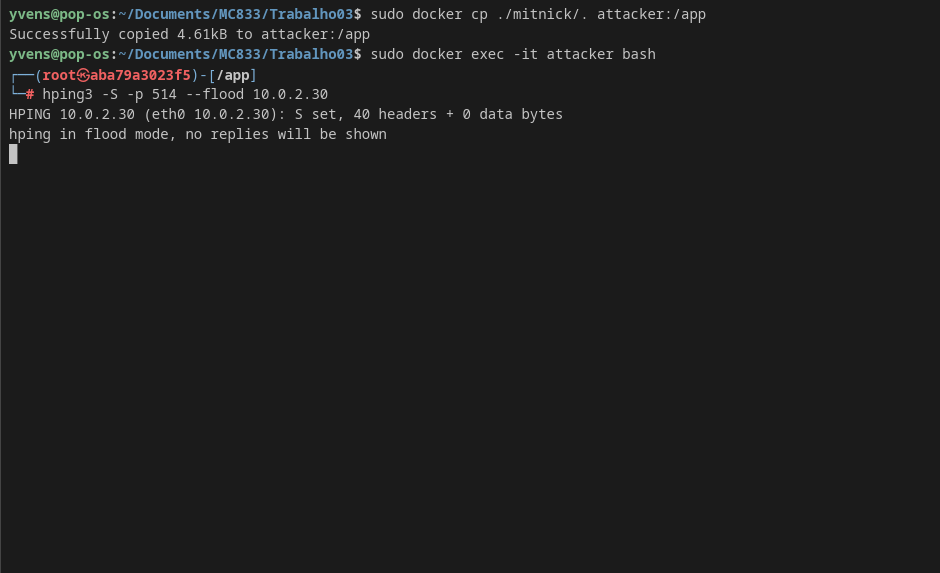
\includegraphics[width=0.8\textwidth]{print1.png}
    \caption{Execução do ataque de SYN Flood utilizando hping3 para silenciar o Servidor Confiável (DoS).}
\end{figure}

\section{Execução do Ataque: Obtenção do ISN e Injeção}
Com o servidor legítimo fora do ar, iniciamos a execução do roteiro principal do ataque, desenvolvido em Python utilizando a biblioteca \textit{Scapy} para a construção e leitura \textit{raw} dos pacotes na rede.

\subsection{Obtenção do Número de Sequência Inicial (ISN)}
Como as máquinas operam em uma topologia de rede local moderna (comportando-se como um \textit{switch} virtual), o tráfego legítimo entre o Alvo e o Servidor não passaria nativamente pela interface do Atacante. Para conseguirmos ler o ISN gerado aleatoriamente, foi fundamental a implementação do \textbf{ARP Spoofing}.

O script injetou um pacote \textit{ARP Request} em \textit{broadcast} informando à rede que o endereço IP do Servidor Confiável (\texttt{10.0.2.30}) agora correspondia ao endereço MAC físico da máquina do Atacante. Ao envenenarmos a tabela ARP do Alvo, garantimos que qualquer resposta destinada ao Servidor fosse enviada diretamente para a nossa interface.

Em seguida, disparamos o pacote \textit{TCP SYN} forjado e ativamos um \textit{Sniffer} assíncrono. Ao receber a requisição de conexão, o Alvo respondeu com o \textit{SYN+ACK}. Devido ao envenenamento ARP anterior, este pacote foi entregue ao Atacante, permitindo ao \textit{Sniffer} capturá-lo e extrair dinamicamente o \textit{Sequence Number} gerado.

\subsection{Conclusão do Handshake, Payload RSH e Validação}
De posse do ISN dinâmico da sessão, o script forjou e enviou unilateralmente o último estágio do \textit{Three-Way Handshake}: um pacote \textit{TCP ACK} com o \textit{Acknowledgment Number} configurado corretamente (\textit{ISN} + 1).

Imediatamente após estabelecer a conexão, despachamos um pacote \textit{TCP PUSH} contendo o protocolo de aplicação RSH malicioso: \texttt{0\char`\\x00root\char`\\x00root\char`\\x00echo + + >> /root/.rhosts\char`\\x00}. A utilização do byte inicial \texttt{0} instruiu o \textit{daemon} RSH a não tentar estabelecer uma conexão secundária de erro via porta \textit{stderr}. Esse comando inseriu a regra de permissão universal (\texttt{+ +}) no arquivo de controle de acesso do alvo.

Conforme demonstrado na Figura 2, após a conclusão do script, a validação foi realizada com sucesso. Com o arquivo \texttt{/.rhosts} manipulado, as restrições de confiança do RSH foram subvertidas, garantindo acesso de superusuário contínuo e irrestrito sem a necessidade de autenticação.

\begin{figure}[H]
    \centering
    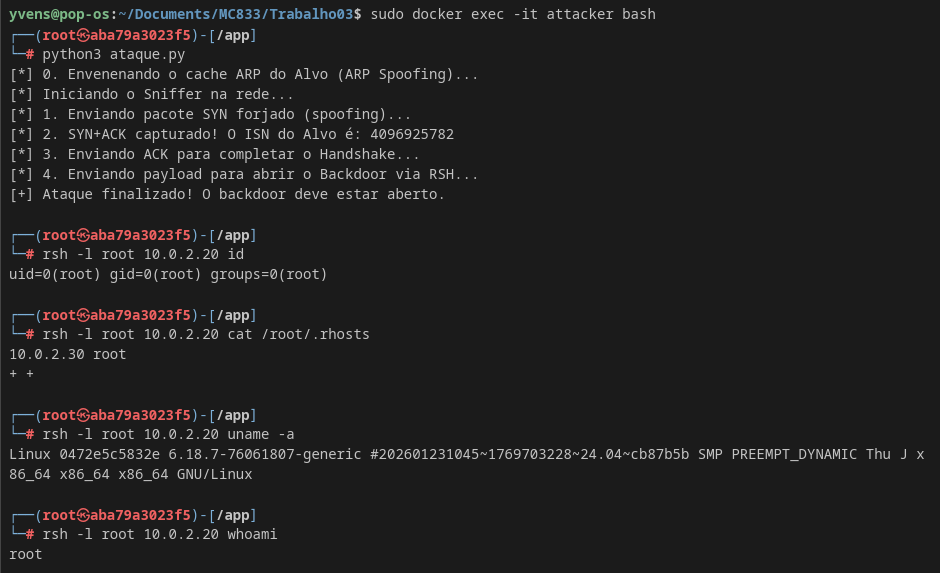
\includegraphics[width=0.8\textwidth]{print2.png}
    \caption{Execução do script em Scapy realizando ARP Spoofing e captura do ISN dinâmico, seguida da comprovação de injeção e acesso irrestrito na máquina alvo.}
\end{figure}

\section{Declaração de Uso de Inteligência Artificial}
Declaro o uso de ferramentas de Inteligência Artificial Generativa como assistentes educacionais para o desenvolvimento desta atividade laboratorial. O auxílio concentrou-se na análise da sintaxe da biblioteca \textit{Scapy} para a forja dos pacotes TCP/IP, na depuração (\textit{troubleshooting}) do comportamento do sistema operacional frente ao envenenamento de tabelas ARP, e na revisão e formatação em \LaTeX\ deste documento técnico. A elaboração das táticas, a execução do ambiente virtualizado e as comprovações práticas de intrusão foram processadas de modo estritamente autoral.

\end{document}